\documentclass[11pt,a4paper]{article}
\title{Behavior Analysis of Elderly using topic models}
\author{Kristin Rieping}
\usepackage[latin1]{inputenc} %andere lettertype
\usepackage{amsmath} %math symbols
\usepackage{amsfonts} %andere font maar wel math symbols
\usepackage{amssymb} % nog meer symbolen
\usepackage{graphicx} %plaatjes toevoegen
\usepackage{fullpage} %minder witte rand
\usepackage{cite} %voor het citeren
\usepackage{caption}
\usepackage{subcaption}

\begin{document}
\maketitle
\pagebreak
\tableofcontents
\pagebreak

\begin{abstract}
The topic model 'Latent Dirichlet Allocation' is applied to real sensor data, that is gained in the homes of elderly people. Different approaches of the models are used to fit the data, including a new developed model. This model encloses a Gaussian Mixture Model into the LDA model, so that the topics are modeled with a Gaussian Distribution. The model parameters are determined with an EM-algorithm.
The goal of this algorithm is to find topics that describe the data in a way, so that it is easily interpretable and usable for different kinds of machine learning techniques that can predict different behaviors.
\end{abstract}


%----------------------------------INTRODUCTION--------------------------------------------
\section{Introduction}
The world population increases unceasingly and besides the percentage of elderly also increases. The manpower to take care of elderly is diminishing. So it becomes more and more important to give elderly the opportunity to live on their own and be more independent of health care. It might be important to monitor elderly in their homes in order to give an alarm if an accident happens or to detect physical and mental declines.

New techniques give the possibility to monitor elderly from the distance or even automatically. Some of these techniques use cameras that are placed in the homes of elderly. But these methods are privacy-sensitive and often not adopted by the elderly.

Other methods use motion sensors that are placed at different locations in the homes of elderly. %find some example
Reading and interpreting this sensor data is often difficult and that is why often activity recognition is done to make the data more readable. But different approaches show that this is also a though challenge.
With many Machine Learning techniques it is also often the case that a lot of annotated data is required.  But the task of labeling a data set is time consuming and can also influence the output of the data while doing so. That is why unsupervised techniques are preferable. Apart from activity recognition we deal with the problem of the representation of the data. From simple motion sensors we receive binary, time sequential data, that is gained over some period of time in the homes of elderly. There are a lot of sensors placed in the houses, which leads to high-dimensional data, that is hard to interpret for classifying algorithms as well as for humans. Finding a correct representation is a challenge.\\

In this thesis we develop an unsupervised algorithm that detects patterns in the data automatically.
In a first step, which is inspired by~\cite{farrahi2008daily}, real live data is used to build a topic model. In a second step a genetic algorithm is used to find the best representation of the data according to the likelihood that is gained from the topic models found in the first step. 
 A topic model in combination with a genetic algorithm might lead to a representation of the data that gives the opportunity to interpret the data more easily and also finds behavior patterns in the data automatically. This furthermore makes it possible to detect deviations in the behavior over a longer period of time. The data that we use is received in the same way as described in ~\cite{van2010activity}, except that our data is not annotated.\\

Topic models are usually used in the field of document classification. The idea is that every document might belong to a couple of different topics and a topic can be described with a distribution over words. A newly seen document can than be assigned to some topics according to the words that occur in the document. The document is than described with a distribution of topics. The topics of a model can be found in an unsupervised manner.
We use this idea to find topics in the given sensor data. So that a day in a persons life can be described with a distribution over topics. And a topic will be described with a distribution over observations. An example of a topic might be 'going to the toilet' or a more global example is 'getting up early'.\\
%%%%%%%%%%%%%%
%Hier nog even kijken
Our data differs from the data that is normally used for this kind of models in some way. For text classification the 'bag-of-words' model is often used, where a distribution of the frequency of words is built. This model is not so easily applicable to the given sensor data, because of the multidimensional and the continuous description of the data. A Text document usually does or does not contain a word of a given dictionary. Therefore our data needs to be discretized in some way.\\
%%%%%%%%%%%%
In a first approach we first simply count the amount of times that a sensor is triggered in a certain window of time. This still produces a broad variety of observations and that is why we cluster the observations with k-means, so that we are able to use the topic model 'Latent Dirichlet Allocation' described in~\cite{blei2003latent}, on our data.\\
In a second approach we develop a topic model based on LDA that models the clusters in the model itself with a Gaussian distribution in every dimension of the observation. In this way the topic model is able to handle high dimensional data. The model parameters are found with an EM-procedure, which uses the likelihood of the model to converge to the optimal model parameters.\\
\\
In the second part of the thesis we use a genetic algorithm to find the best representation of the data.
Earlier we described the part of discretization the data in some way. Choosing the correct length of a time-interval, in which the sensor activities are counted, might be hard. There are also plenty of other variables to choose, that lead to a different representation of the data. For example we can choose to group all sensors together that are in the same room of the house. But we cannot be sure that this leads to a better representation of the data. Further there are different kind of sensors placed in the houses and we might want to distinguish between these sensors, so that a different weight is given while counting an activity. For example an activity at a door sensor might give more information of a persons behavior then a motion sensor, which is triggered more often also by small, not that important movements. It might also a good idea to look at the transition of the observations, so given an observation, what are the observations before and after this one.\\
So the representation of the data depends from a lot of different variables. This variables are optimized with a genetic algorithm. The log-likelihood, from the previously derived topic models, is used as the fitness function of the genetic algorithm.\\

In the next chapter of this thesis we give an overview of related approaches. In section \ref{sec:DataDesc} we describe the data that we use in more detail. This is followed by section \ref{sec:TopicModels} which describes the two different ways of the usage of Topic Models with our data. In section \ref{sec:features} we describe the different ways of feature representation of our data and also show how the genetic algorithm is used. The section \ref{sec:Experiments} we describe the different experiments that we perfomed. We finalize the thesis with the section \ref{sec:DisCon}.


%  Instead of a bag-of-word model that describes our data, every observation is model with a Gaussian Distribution in every dimension.
% 
% 
% In a second step a genetic algorithm is used to find the best feature representation of the data. The data is discretized in times-slices and divided into different fields. The likelihood of the EM-algorithm of the topic model is used as a fitness function. In this way the best representation of the data can be found.\\ 
% Ik weet nog niet hoe ik dat precies doe, dus maar nog niet meer omschrijven.
% Together this two steps might give a good indication how this kind of data can be efficiently used with other machine learning techniques.
% This data also might give valuable information to health proffesionals. The topics described in the first step might give a good indication of the health of the elderly.
% 
% It might be possible to predict the health of a person and give additinal health care if needed.


\section{Related Work}
In the work of Casale~\cite{Casale:2009} continuous data is modeled with a the topic model LDA. The words for the topic models are generated by clustering the data. Two different cluster methods are used, K-means and mean-shift.



%--------------------------------DATADESCRIPTION--------------------------------------------
\section{Data Description}
\label{sec:DataDesc}
In this section we describe in what kind of houses the data is gathered and what kind of persons live there. We describe the sensors that are used and give an impression of the data that is received from this sensors.
\subsection{Homes and persons}
In the homes of five different people sensors are installed. The floor-plan of these homes is for all residents the same and is shown in figure ...(hier zou ik graag een plaategrond van de woningen willen toevoegen als dat mogelijk is) There might be small differences of the locations of the sensors due to the personal arrangements of peoples stuff.
The persons that live in the homes are people that need healthcare on a regular basis, but they are further able to live on their own. The amount of data gained differs but there is at least fifty days of data available for every person. 
\subsection{Sensors}
There are two different types of sensors installed in the homes, reed- and motion-sensors. The reed-sensors which are mostly installed at doors get the value 'one' if a door is opened and the value 'zero' if the door is closed again. The toilet flush has also a reed sensor. (A float sensor??)
The motion-sensor are placed at different places in the homes, mostly against the walls. They have a range of ... meters. If a motion occurs in the region of a sensor the value of the sensor becomes 'one' and 'zero' again immediately. After that the sensor is set to mute for about 3 minutes (or is this 1 minute), which means that in this time there is no motion captured. This is done to avoid constantly firing of the sensor, which would lead to superfluously activity encounter.
The sensors are listening continuously.

\subsection{Received Data}
In figure ~\ref{fig:PlaineSensorData} an example of the received data is given. There are two hours of one day shown for one person. Several sensors that are located in the same room are manually grouped together in a field. The fields are $\{$'kitchen', 'living room', 'bathroom', 'bedroom', 'hallway'$\}$. They are marked in the figure with different colors.

\begin{figure}[h!]
  \centering
  \begin{subfigure}[b]{0.45\textwidth}
    \centering
    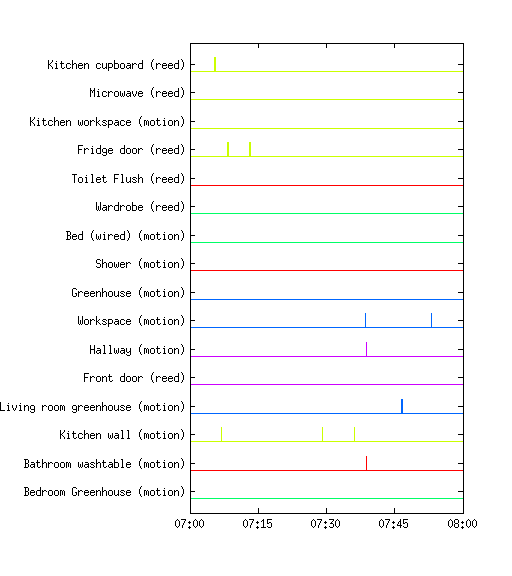
\includegraphics[width=\textwidth]{Pictures/SensorsMorning.png}
  \end{subfigure}
  ~
  \begin{subfigure}[b]{0.45\textwidth}
    \centering
    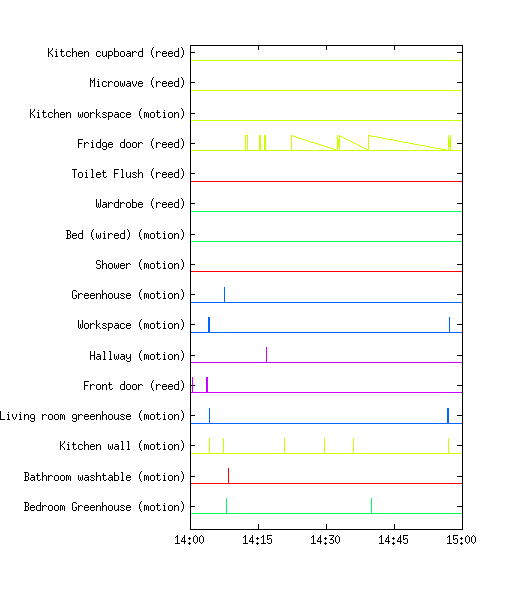
\includegraphics[width=\textwidth]{Pictures/SensorsNoon.png}
  \end{subfigure}
  \caption{Sensor Data for two different hours at a day of one person. The fields `kitchen`,'living room','bathroom','bedroom','hallway' are marked with the colors 'yellow','blue','red','green','purple' respectively.}
  \label{fig:PlaineSensorData}
\end{figure}

In the figure you can see that at noon the fridge is used, but the sensor data is not captured correctly. This errors needs to take into account when dealing with the data. Other problems that occur are that one sensor is not working because it is not well connected or the batteries are empty. It also happens that the network is not working or the network cable is pulled out, which means that the data cannot be send to the server that stores the data. These kind of errors need to be handled manually and are not taken into account when modeling the data.

In the following approaches we only take the amount of times into account how often a sensor is triggered. The length on how long a sensor has the value one is not taken into account.
The data is discretized in some way, because we only count the amount of times a sensor is triggered. The amount of time that a sensor has the value one is not totally taken into account in our model
THIS NEEDS TO BE MENTIONED SOMEWHERE. I am not totally sure if this is the correct place though.

\pagebreak
%-----------------------------------TOPICMODEL----------------------------------------------
\section{Topic Models}
\label{sec:TopicModels}
In the introduction of this section we describe the general idea of topic models followed by a section that describes how this kind of models can be used on the sensor data that we have. After that we introduce the extension of the LDA model which combines the clustering and topic estimation in one algorithm.

\subsection{Introduction to Topic Models}
Topic models are often used in the field of document classification. Given a set of documents (corpus) it is assumed that every document belongs to one or more topic(s). So for example a news article may belong for some percentage, let us say 30 \%,  to the topic 'Economy' and for 70 \%  to the topic 'Politics'. Another document of the same Corpus may belong to the topic 'Economy' with 50 \%, 'Politics' with 30 \% and 'Global Warming' with 20 \%. There might be a lot of different topics and the topics can have different level of details. 
\\
The topics are defined by several words that can occur in the documents. The topic 'Economy' may be defined by the list of words \{'trade', 'industry','GDP'\}. Other topics have different lists of words that describe them. The list might be longer or shorter and the words in the list will depend on the corpus that is used to generate the topics. It might also be the case that one word belongs to multiple topics. Eventually we can find the topic distribution of a document according to the words that are included in this document.\\
In the topic model 'Latent Dirichlet Allocation' (LDA) it is assumed that a Corpus can be made out of a generative process. The parameters that generate the corpus are than used to describe the model of the corpus. The generative process which builds a corpus is as follows:
\\
For every document that is generated in the Corpus
\begin{enumerate}
 \item Choose the amount of words in the document from $N~Possoin(\xi)$.
 \item Choose a topic distribution $\theta \sim Dir(\alpha)$ for the document.
 \item For each of the N words $w_n$:
 
 \begin{enumerate}
  \item Choose a topic $z_n \sim Multinomial(\theta)$.
  \item Choose a set of words $w_n$ from the set of all words $V$ from $p(o_n |z_n;\beta)$, a multinomial probability conditioned on the topic $z_n$. Where $\beta$ is the distribution over words given a topic.
 \end{enumerate}

\end{enumerate}

The model is also shown in figure~\ref{fig:modelBasic}. The parameters $\alpha$ and $\beta$ define a corpus.

\begin{figure}[h!]
\centering
\def\width{0.7 \textwidth}
\input{Pictures/ModelBasic.pdf_tex}
\caption{Graphical representation of the LDA model}
\label{fig:modelBasic}
\end{figure}

To determine the model parameters an EM-algorithm can be used. How this algorithm can be applied is extensively described in~\cite{blei2003latent}. \\
In the next section we describe how this model can be used with the sensor data, that is gained in the different houses.


\subsection{Topic models with Sensor Data}

In order to employ the topic model with the sensor data we first introduce the different levels of description given our data and relate them to the terms of document classification.
\begin{itemize}
 \item \textbf{Dataset/Corpus}: One dataset $C$ describes the sensor data that is gained in the home of a single person. So for every person there is a separate dataset. This set of data can be compared with a Corpus in document classification.
 \item \textbf{Day/Document}: Every Dataset is divided in days. A day can be compared with one document in a Corpus.
 \item \textbf{Observations/Words}: Finally every day is build of a set of observations. The amount and dimension of the observations depend on the representation of the features, which is described later in chapter \ref{sec:features}. Observations can be roughly compared with words in document classification.
\end{itemize}

There are some differences between the data that is used for topic detection in documents and our sensor data.\\
The main difference is that words that look similar to each other, like "illusion" and "allusion", may belong to a totally different topic in the document classification. But in our case, two observation that are similar to each other, are more likely to refer to the same topic. So for example if the topic "preparing food" has the observation using fridge 3 times in it, an observation of using fridge 4 times may also refer to the same topic. That is why we cannot directly compare the words in a text document with the observations used in the sensor data.\\
Another difference is that in the topic model, LDA, it is assumed that the order of the words, in that they appear in the text, does not matter. In our case the time when an observation is made is of big influence. We can overcome this problem by adding time as an additional dimension to our observations.
\\

If the Bag-of-Words model will be applied to the data, a dictionary of all unique observations must be made. All this observations then will be seen independent from each other. This is shown in figure~\ref{fig:FSBOW}. Observations that are assigned to the same topic do not need to lie close to each other in the feature space and the correct topics might not be found with LDA.

\begin{figure}[h!]
\centering
\begin{subfigure}[b]{0.3\linewidth}
\centering
\def\svgwidth{140pt}
\input{Pictures/BOW.pdf_tex}
\caption{The Bag-of-words model with topic assignment.}
\label{fig:FSBOW}
\end{subfigure}
~
\begin{subfigure}[b]{0.3\linewidth}
\centering
\def\svgwidth{140pt}
\input{Pictures/kMeans.pdf_tex}
\caption{Feature space with k-means and topic assignment.}
\label{fig:FSk-means}
\end{subfigure}
~
\begin{subfigure}[b]{0.3\textwidth}
\centering
\def\svgwidth{140pt}
\input{Pictures/GMM.pdf_tex}
\caption{Gaussian Mixture Model with LDA}
\label{fig:GMM+LDA}
\end{subfigure}
\caption{The two different topics are marked with red and blue.}
\end{figure}

To make sure that similar observations will be grouped together and will appear in the same topic, we can apply the k-means algorithm to find clusters in the data. The centroids of the clusters then function as 'words' and can be used in the same way as text data. So if we apply LDA to the clustered data some clusters may fall into the same topic. This is shown in figure ~\ref{fig:FSk-means}.\\
The downside of the k-means clustering approach is that clustered are separated with a hard line and that you have to choose the number of clusters $k$ in advance. A better approach would therefore be a Gaussian mixture model. And instead of defining the clusters by forehand we will let the topic model determine the priors of the clusters itself. In this way it might be possible that the topic model will find a better descriptions of the topics. This is shown in figure~\ref{fig:GMM+LDA}.



% 
% Let us say we have a two dimensional feature space. For example we only have two sensors in our data, than every dimension will refer to one of the sensors. A representation of this model is shown in figure bla (a). A cross marks an observation and is seen as a new 'word' in the bag-of-word method. We can use this data with the LDA model. The problem only with this approach is that similar observations are not group together and it might be possible that a similar observations are not grouped together in the same topic when we apply the LDA model.

% 
% 
% If we cluster the observations on forehand with a the k-means algorithm we can reduce the size of the dictionary (which contains all unique observations) and use again the LDA method to find the topics. The problem here is that there is a hard separation line between the clusters as is shown in figure bla (b).
% 
% So we invented a third method which is a kind of gaussian mixture model included into the LDA topic model. So instead of cluster the model with priors from the data itself we relate the priors directly to the topis and combing the part of clustering and the deriving the topics in one algorithm. In this way clusters are grouped together directly if they belong to the same topic, as is shown in figure bla (c).
% 
% 
% 

% 
% 
% In the next two sections we describe the two different ways how we use the topic models with our data. First we describe the combination of k-means clustering and the basic LDA model as it is described in [Blei]. And after that we describe our new approach that combines the clustering and topic modelling in one algorithm. In this algorithm we step away from the bag-of-words model representation of the data.
%  Nog toevoegen dat we twee manieren gaan gebruiken(LDAbasic and LDAext)
% %%TOT HIER!
% 
% 

%   \subsubsection{K-means}
%  In the previous section we addressed the problem of a wide variance of observations. With a bag-of-words model, as it is used in the LDA approach, similar looking words/observations are not likely to be put in the same topic. All observations, that are not exactly the same, are independent from each other and may not lead to the same topic. Because of the low amount of training data it is not very likely that the same observation will be seen often enough to learn topics from the data properly.
% That is why we need to reduce the amount of unique observations and group similar observations together. In terms of document classification, we could say that we need to reduce the size of the dictionary.


% In a first-approach we use k-means clustering to reduce the size of the dictionary, which is the set of all observations that can be found in the data.
% We do not use the time dimension for the clustering part, because this would compromise our data so that clusters are not detected properly. We use the euclidean distance to determine the best mean.
% 
% maybe preprocess the data with coarse grain time dimension
% 
% size of the dictionary
% is it the case that with a lot of data simialar looking words will be put in the same topic? Or will it just be a different topic?
% 
% 
% 
% In our data the size of the dictionary, which contains all unique observations in the whole corpus is relative large with respect to the size of the data that we have. There are a lot of different observations that are similar to each other, but differ only in one value of the 6 dimensions. So for example the observation $o_1=\{1 ,2 ,5 ,3,14\}$ is similar to the observation $o_2=\{2 ,2 ,5 ,3,14\}$. The only difference of sensor activities is in the first field. In the LDA model these two observations/words will be seen as two different dimensions and the similarities are not captured. In fact a lot of words will only be seen once in the whole corpus and finding good parameters is not possible.
%  So we need to find a way to capture similar observations to build a proper topic model. A simple way is to cluster all observations together and then use the EM-algorithm to estimate the parameters of the  LDA model.
%  For the clustering part we used the k-means algorithm. We reduced the size of the dictionary to 20. After that we use the EM-algorithm as described above.
%  In the clustering we leave out the time dimension because this is fucking up the clusters
 
%   \subsubsection{Latent Dirichlet Allocation with clustered Data}
% The generative model 'Latent Dirichlet Allocation' [Blei] is a way to describe a topic model. In this model it is assumed that a Corpus can be generated from a distribution of topics, where every topic can be represented with a distribution of words. In our case the documents are days and the words are observations $o_n$. In the previous section we described how we reduced the size of the dictionary $V$.
% The generative process that would create the data will look like this:
% 
% For every day that will be generated:
% \begin{enumerate}
%  \item Set the amount of observations in every document to size N (for every day the same amount).
%  \item Choose a topic distribution $\theta \sim Dir(\alpha)$ for the day.
%  \item For each of the N observations $o_n$:
%  
%  \begin{enumerate}
%   \item Choose a topic $z_n \sim Multinomial(\theta)$.
%   \item Choose a set of observations $o_n$ from the set of all observations $V$ from $p(o_n |z_n;\beta)$, a multinomial probability conditioned on the topic $z_n$. Where $\beta$ is the distribution over observations given a topic.
%  \end{enumerate}
% 
% \end{enumerate}
% %!!!Describe the model variables!!!!!
% 
% With the assumption that the data that we got from the sensor system has the same structure than the data created with the generative process we can find the model parameters $\alpha$ and $\beta$ for LDA with the EM-algorithme described in \cite{blei2003latent}.

\subsection{LDA-Gaussian Model}
In this section we explain how the part of clustering is combined within the LDA model itself. Instead of the k-means clusters we use a gaussian distribution to model every dimension within the features.


  \subsubsection{Motivation and Assumptions of the Model}
  
In the previous section we clustered the data first with k-means and then used the LDA model to determine the topics of the model. This approach has some drawbacks. First of all the clusters that are found with k-means have a hard separation lines between the clusters. No quality measurement on the clusters is given and every point that falls in the cluster belongs to the cluster with the same probability, no matter how far it is away from the mean. Also every cluster has the same weight so there is no distinction between the clusters.

With a Gaussian Mixture Model we might be able to distinguish between more or less important clusters. But we might want to let the topic model decide which topics have more influence and which not according to the data.\\
That is why we combined the clustering part and the topic estimation into one step. Instead of a multinomial distribution over the bag-of-words model of the observations given a topic, we model a Gaussian distribution over every dimension of the observations. In this way similar observation can be captured in the model itself and are not generalized in a cluster.\\
The difference is that instead of a large, fixed set of unique observations (Dictionary), with a multinomial distribution, instead we take a Gaussian distribution over every dimension of the observations. In this way smoothing is not necessary, because unseen observations will be handeled properly.
In the next sections we describe the model in more detail. We first give an overview of the generative process. Then we explain the variational inference that is necessary to make the parameter estimation possible. And finaly explain the EM-algorithm that determines the parameters.

Every topic will have its own distribution over the dimensions. A
topic can be described as shown in figure %\ref{fig:topic}.
In this figure an example of a topic description is shown
% \begin{figure}
%  \includegraphics[\width=\textwidth]{Pictures\topics.png}
%  \caption{An awesome topic}
%  \label{fig:topic}
% \end{figure}

  \subsubsection{Model Description}
   meer uit de zicht het bestaat en het wordt niet gegenereerd.
  
  Our model assumes that every day in a dataset can be represented as random mixtures of latent topics, where every topic can be described as a distribution over observations. We assume the following generative procss for every day $m$ in $M$:
\begin{enumerate}
 \item The amount of observations on a day $m$ is fixed with size $N$ (for every day the same size).
 \item A distribution over the topics $\theta \sim Dir(\alpha)$ for that day.
 \item For each of the N observations $o_n$:
 
 \begin{enumerate}
  \item Estimate the topic $z_n \sim Multinomial(\theta)$.
  \item An obeservations $o_n$ is generated from $p(o_n |z_n,\boldsymbol\mu,\boldsymbol\sigma)$, a probabilty which can be drawn from a set of Gaussian distributions, which are conditioned on the dimension $d$ of the observation and the topic $z_n$. $\boldsymbol\mu$ and $\boldsymbol\sigma$ are two matrices of size  $D\times k$, which represent the mean and standard variance of the Gaussian distribution.
 \end{enumerate}

\end{enumerate}
  
In this model the amount of topics $k$ is assumed to be known and fixed and with it the size of the topic variable $z$.
 Here is the gaussian shit varibale description.
The probability for the observations is parameterized with two matrices $\boldsymbol\mu$ and $\boldsymbol\sigma$, both of size $D\times k$, where $D$ is the amount of dimensions in an observation and $k$ the amount of topics. They present the mean and standard deviation respectivally and for every topic $i$ and every dimension $d$ there is a set of parameters, which describes a Gaussian distribution.  Every value of a dimension for an observation $o_{ndi}$ can then be drawn from a Gaussian Distribution $\mathcal{N}(\mu_{di},\sigma_{di})$.
The size of the dimension $D$ is assumed to be fixed and a more extensive description of the representation of the observations is given in section \ref{sec:features}. $\alpha$ represents the Dirichlet parameter and is vector of length $k$.
Alpha beter uitleggen
the variable $\alpha$ represents the Dirichlet Parameter
$\alpha$ is a vector of length $k$.
Misschien hier ook het grafische model. Of toch misschien al eerder? Nee denk het niet, want als je het model alleen ziet dan weet je niet wat alles betekend. Dus het grafische model moet nu komen.

Given the parameters $\alpha$, $\mu$ and $\sigma$, the joint distribution of a topic mixture $\theta$, a set of $N$ topics $z$ and a set of $N$ observations $o$ is given by:
\begin{equation}
 p(\theta,\textbf{z},\textbf{w}|\alpha,\mu,\sigma) = p(\theta|\alpha) \prod_{n=1}^N p(z_n|\theta) p(w_n|z_n,\mu,\sigma)
\end{equation}


%A visualization of this model is shown in figure \ref{fig:modelExt}.
%
%\begin{figure}[t!]
%\centering
%\def\svgwidth{0.8\textwidth}
%\input{Pictures/ModelExt.pdf_tex}
%\caption{Graphical representation of the LDA model}
%\label{fig:modelExt}
%\end{figure}
%

  
Assuming that the generative process described above can describe the available data properly, we now want to find the parameters so that the model best describes our data. We want in fact maximize the probability for the dataset $C$ given the model with respect to the parameters $\alpha$, $\mu$ and $\sigma$. This probability looks like this
\begin{equation}
p(C|\alpha,\mu,\sigma) = \prod_{m=1}^M p(m|\alpha,\mu,\sigma)
\end{equation}
where $M$ is the amount of days within the dataset and the probability for a day $m$ given the three parameters, which is the marginal distribution over a day, is
\begin{equation} 
p(m|\alpha,\mu,\sigma) = \int p(\theta|\alpha)  \left( \prod_{n=1}^N \sum_{z_n} p(z_n|\theta) p(w_n|z_n, \mu,\sigma)  \right) d\theta
\end{equation}
This distribution is gained by integrating the joint distribution by $\theta$.
In the next section we describe how we find the optimal parameters.



  
\subsubsection{Variational Inference}
 
Thie marginal distribution can be written in terms of the parameter $\alpha$, $\mu$ and $\sigma$ as
  \begin{equation}
   p(m|\alpha,\mu,\sigma) = \frac{\Gamma (\sum_i \alpha_i)}{\prod_i \Gamma(\alpha_i)} \int \left( \prod_{i=1}^k \theta_i^{\alpha_i-1} \right)
   \left( \prod_{n=1}^N \sum_{i=1}^k \prod_{d=1}^D \theta_i \mathcal{N}(o_{nd},\mu_{id},\sigma_{id} ) \right)
  \end{equation}
Due to the coupeling between $\theta$ and the Gaussian parameters $\mu$ and $\sigma$ this probability is intractable to compute. That is why we use a convexity-based variational algorithm to approximate the loglikelihood of a given dataset. 
An approximation of the model is given with 
  \begin{equation}
   q(\theta,z|\gamma,\phi) = q(\theta|\gamma) \prod_{n=1}^N q(z_n|\phi_n).
  \end{equation}
In this model $\gamma$ represents the Dirichlet parameter and $\phi$ are the multinominal parameter which can be viewed as the probabilty $p(z_i|o_n)$ and is given as a $k \times N$-matrix for every day $m$. The graphical representation of the model is shown in figure \ref{fig:ModelApprox}.
  
%  
%\begin{figure}[t!]
%\centering
%\def\svgwidth{0.4\textwidth}
%\input{Pictures/ModelApprox.pdf_tex}
%\caption{Approximation of the model}
%\label{fig:ModelApprox}
%\end{figure}
%  
  
  
  
  Given the variational distribution we can estimate the lower bound of the loglikelihood with the Jensen inequality as
  \begin{equation}
   \begin{split}
    L(\gamma;\phi;\alpha;\mu;\sigma) =& E_q[\log p(\theta|\alpha)] + E_q[\log p(\textbf{z}|\theta)] + E_q[\log p(\textbf{w}|\textbf{z},\mu,\sigma)] \\
   & -E_q[\log p(\theta)] - E_q[\log q(\textbf{z})]
   \end{split}
  \end{equation}

In terms of the model parameters and the variational parameters this becomes
\begin{equation}
  \begin{split}
 L(\gamma;\phi;\alpha;\mu;\sigma) =& \log \Gamma (\sum_{j=1}^k \alpha_j) - \sum_{i=1}^k \log \Gamma(\alpha_i) + \sum_{i=1}^k (\alpha_i-1)(\Psi(\gamma_i)-\Psi(\sum_{j=1}^k \gamma_j)) \\
 & + \sum_{n=1}^N \sum_{i=1}^k \phi_{ni} (\Psi(\gamma_i)-\Psi(\sum_{j=1}^k \gamma_i)) \\
  & + \sum_{n=1}^N \sum_{i=1}^k \sum_{d=1}^D \phi_{ni} \log( \mathcal{N}(o_{nd};\mu_{id},\sigma_{id})) \\
  & - \log \Gamma (\sum_{j=1}^k \gamma_j) + \sum_{i=1}^k \log \Gamma (\gamma_i) - \sum_{i=1}^k (\gamma_i -1)(\Psi(\gamma_i)-\Psi(\sum_{j=1}^k \gamma_j)) \\
 & - \sum_{n=1}^N \sum_{i=1}^k \phi_{ni} \log \phi_{ni}
  \end{split}
  \label{eq:likeli}
\end{equation}
With an EM process we are then able to maximze this lower bound on the loglikelihood. The two steps are:
  \begin{enumerate}
   \item \textbf{E-step:} For each day $m$, optimize the variational parameters $\{ \gamma_{m}*,\phi_{m}* \}$
   \item \textbf{M-step:} Maximize the resulting lower bound on the loglikelihood with respect to the model parameters $\alpha$, $\mu$ and $\sigma$.
  \end{enumerate}
  
  We now give a more detailed description on both of these steps.
  
  \paragraph{E-step}
In the e-step of the algorithm the variational parameters $\phi$ and $\gamma$ are optimized. To get the update function for $\phi$ we get all terms of the lower bound of the loglikelihood in equation (\ref{eq:likeli}) that contains the variable $\phi$. 
Take $y_i=\sum_{d=1}^D \mathcal{N}(o_{nd};\mu_{id},\sigma_{id})$
We add the constraint $\sum_{i=1}^k \phi_{ni}=1 $ to the formula and get
\begin{equation}
 L_{[\phi_{ni}]} = \phi_{ni}(\Psi(\gamma_i)-\Psi(\sum_{j=1}^k \gamma_j)) + \phi_{ni} \log(y_i) + \lambda_n(\sum_{j=1}^k \phi_{ni} -1)
\end{equation}
From this equation we take the derivative of the formula and set it to zero. This leads to the first update function
\begin{equation}
 \phi_{ni} \propto \log(y_i) \exp(\Psi(\gamma_i) - \Psi(\sum_{j=1}^k \gamma_j))
\end{equation}
\\
For $\gamma$  we also take all terms of equation \ref{eq:likeli} that contain this variable and set the derivate to zero. This leads to the second update equation
\begin{equation}
 \gamma_i = \alpha_i + \sum_{n=1}^N \phi_{ni}
\end{equation}

  Nu nog de algorithme geven

  \paragraph{M-Step}
  
In the m-step the parameters of the Gaussian distribution $\mu$ and $\sigma$ are estimated with the weighted arithmetic mean calculated over all observation in a dataset given the parameter $\phi$, which is gained in the previously e-step. This leads to the update formulas
\begin{equation}
 \mu_{di} = \frac{\sum_{m=1}^M \sum_{n=1}^N o_{dn} \phi_{ni} }{\sum_{m=1}^M \sum_{n=1}^N  \phi_{ni}}
\end{equation}
and
\begin{equation}
 \sigma_{di} = \sqrt{\frac{\sum_{m=1}^M \sum_{n=1}^N o_{dn}^2 \phi_{ni} }{\sum_{m=1}^M \sum_{n=1}^N  \phi_{ni}} - \mu_{di}^2}
\end{equation}
\\
To calculate the parameter $\alpha$ we again take all terms of the likelihood that contains the variable $\alpha$. The derivative in the Hessian form is
\begin{equation}
 \frac{\partial L}{\partial \alpha_i\alpha_j} =  m(i,j) M \Psi'(\alpha_i) - \Psi'(\sum_{j=1}^k \alpha_j)
\end{equation}
On this equation we can use the Newton-Rhapson method to calculate the optimal $\alpha$.



% For a reason 
% the reason is that lda captures priors for the days, that are given with the 
% which is still not is clear for me, we combine the clustering and determining of the topics in one algorithm.
% Preprocessing the data with k-means may not capture the topic distributions probably. The time dimension is not taken into account in the clustering part. So we want to avoid the preprocessing the data with k-means and add the the clustering part directly in the model.
% So first we describe how the model will change with respect to the LDA model descriibed above (or maybe: ... how extension of the LDA model looks like) and we also describe how the parameters are determined with the EM algorithm.
% 
% 
% So what is different? Maybe do not ask this question but just explain how the model looks like.
% 
% The main change of the model is that it is also captures similar observation in one topic.
%  So instead of describing a topic only with one discrete value in one dimension, we model every dimension in the observation with a Gaussian distribution. So every dimension given a topic needs to be defined with a mean and a standard deviation. The dimension might depend from each other
% 
% 
%   This is done in the following way:
% Instead of storing the probability for a observation given a topic, which is done in the matrix $\beta$, we assume that every dimension of the observations is normal distributed given a topic. So we store the mean and variance for every dimension given a topic in two matrices of size $d \times k$ where $d$ is the dimension of the observations and $k$ the amount of clusters. For now we assume that the dimensions of the observations are uncorrelated. The EM-algorithm is adjusted to calculate the $\beta$- matrix properly.
% 
% - The combination of the k-means clustering and the LDA model might not capture the topics correctly. The k-means clustering gives a hard boundaries on the words, which is also a drawback from the sequential combination of clustering and topic estiamtion. Therefore we want to comine these two step in one.




%--------------------------------------FEATURES----------------------------------------------
\section{Features}
\label{sec:features}
The plain data that is gained from the sensors needs to be discretized in some way so that it can be used in the topic models. So first we group all sensors together that belong to the same field. One day is than devided into timeslices of length $l$. In first instance we take $l=30$, which means that there are 48 timeslices on a day. A day starts at 3 a.m. in the morning so that we reduce the chance to cut between activities. It still can occur that a person goes to bed late or that he needs to visit the toilet, but we will ignore this fact for now.\\
In every time-slice of a field we look at the amount of times that a sensor in this field is activated and count this activities. So we do not look at the length of time that a sensor stays in the active state, but only how often it changes into the active state. So given five fields for one day we have 48 observation $o$ where every observation has five dimension. We do not take the length of the sensor activity into account because this sometimes can lead to unrealistic high values. These values can occur if someone leaves a door open of a cupboard open for example. Then the observations contains a high value but does not contain a lot of information about the behavior. In figure \ref{fig:FeatEx} %Give an example.
EXAMPLE\\
This is the simplest way to use the data, but there are plenty of different ways to combine the time-slices. So for example we can change the size of the time-slices, which leads to a higher resolution and may give more detailed information. Another way to get a different feature representation is to combine sequential time-slices. So for a given time-slice add the values of the previous and the subsequent time-slice, that will lead to a 15 dimensional observation. In this way the transitions are taken more into account, which might contain valuable information over the behaviour.\\
We also might want to combine different sizes of time-slices into one observations, so that the global and detailed view is combined.\\
You can see that there are plenty of different ways to use the data and finding the best feature representation is a big challenge. What the best feature representation is depends also on the usage of the data. A system that wants to detect the activities might a more detailed feature representation. But a system that only monitors the health of a person might only need a global feature representation.

% Wat hoort hier in te staan???
- data wordt ingedeeld in fields, deze is afhankelijk van de locatie van de sensor
- alle observaties in een field worden samen bekeken
- een dag wordt ingedeeld in timeslices
- the amount of timeslices is variable
- we count the amount of 1's in one timeslice of a field
- there are a lot more different ways to use the data
- we can combine different timeslices, so maybe the best topics are found if their are different timeslice widths are combined.
- another way to combine the timeslices is to look at the previous and the subsequent timeslice and combine the three observations of this timeslices into one big observation. In this way the transitions are captured well.
- We also may want to look at the way the different sensors in the homes are handled. A reed sensor might be much more important than a motion sensor. The reed sensor is mostly connected to doors and opening the fridge might be of more information than if a person only moves in the living room, this might be only be caused by someone who shifted a little bit on the couch. 




% Waarvan is het afhankelijk????
% Waarschijnlijk of ik een experiment kan runnen en hoe ik dan aanpak.



% In a first approach we discretize the data into time-slices of half an hour. In each time-slice we count the amount of sensor activations in all the fields. We differentiate between two different kind of sensors. For the reed sensors, which are installed at doors and the toilet flush, we count every change of sensor value. So open and close a door is both count as an activity.\\
% %How is the toilet sensor been seen? 0 and 1?
% The motion sensor can sens a new motion every minute. But in between the sensor will still have the same value, which is 1. That is why we count for every minute the sensor has the value 1 a new activity. So if the sensor has the value 1 for three minutes, we count three activities for the particular sensor.\\
% The amount of activities captured at every sensor is add together for every field. So every time-slice can be represented as a vector $w_n$ of length five, for every field a value $v_i>=0 \in \mathbb{N}$. We add an additional dimension to the vector to capture the the time in which the observation is taken. The values lay between 1 and 48, for every time-slice a value. This is necessary to model the time dependency from the data, which is not automatically captured in the topic model that we are going to use. We say that a day starts at 3 a.m. so that we reduce the chance to cut between activities. It still can occur that a person goes to bed late or that he needs to visit the toilet, but we will ignore this fact for now.
% 

%----------------------------------------EXPERIMENTEN-----------------------------------------
\section{Experiments}
\label{sec:Experiments}

\subsection{Experiments with the Topic models}
To test the performance of the topic models we set the features to a fixed value. The sensors are divided in the five fields $\{$'kitchen', 'living room', 'bathroom', 'bedroom', 'hallway'$\}$. The size of the time-slices is 30 minutes, which means that a day is divided into $N=48$ observations. A day starts and ends at 3 am. An observation has six dimensions, five dimensions for the different fields and one dimension for the time value in which an observation occurs. In the basic LDA model we use a coarse grain value for the time. This means that the sixth dimension can have 5 different values, where the time intervals are $\{ 3am - 8am, 8am - 1pm, 1pm - 18pm, 18pm - 23pm, 23pm - 3am  \}$.
\subsubsection{Visualization of the Topics}
\paragraph{k-means and LDA}
Hier het best de clusters en ook de topics visualizeren
clusters visualizeren is nog wel te doen. Vraag is of deze ook wel consistent blijven.

\paragraph{LDA extension}
We used 20 topics to run the LDA-Gaussian model. The 10 topics with the highest alpha value are shown in figure ~\ref{fig:TopicVisu}

\begin{figure}
 \centering
 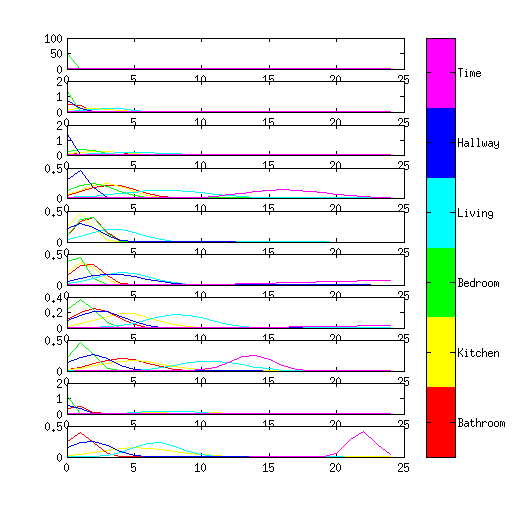
\includegraphics[width = 0.7\textwidth]{Pictures/TopicVisuLDAext1.png}
 \caption{The 10 topics with highest alpha values. Every field is given in a different color.}
 \label{fig:TopicVisu}
\end{figure}

NOTE:
De plot kan denk ik nog beter. Ik denk dat ik de tijd van de andere observaties moet scheiden. De y-as verschillt voor de verschillende topics. Een 'field' wordt niet getoond als de variantie te klein is. Ik moet nog even bedenken wat ik daarmee doe.


\subsubsection{Perplexity of the topics}
We wish to find a high loglikelihood on a hold-out-set, so that we can be sure that the model does not over-fit on the training data. So we calculate the perplexity of this set with

\begin{equation}
 perplexity(D_{test}) = exp \left\{ - \frac{\sum_{d=1}^M \log p(\textbf{o}_d ) }{M*N} \right\}
\end{equation}

In figure ~\ref{fig:Perplexity} the Perplexity for the Hold-out-set is shown for the data gained in one House. We take the mean over ten runs. 10\% of the data is used as a hold-out-set. We initialize the EM-algorithm with 5 random days of the training data.

\begin{figure}
 \centering
 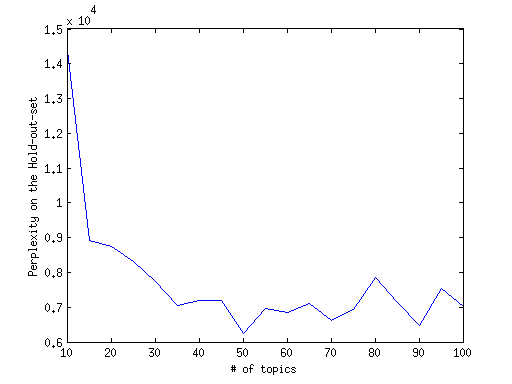
\includegraphics[width = 0.7\textwidth]{Pictures/OutcomeExp4.png}
 \caption{Perplexity (x-axis) for the hold-out-set for different amount of topics (y-axis)}
 \label{fig:Perplexity}
\end{figure}

NOTE:
Kijken of ik hetzelfde voor k-means kan doen. De likelihood kan ik niet direct met elkaar vergelijken, maar wel met de BOW model. Ik moet het ook nog even voor de andere huizen runnen.

% \subsubsection{Variation of initialization}
% 
% worden de zelfde topics altijd weer gevonden of varieert dat heel erg. (hoe kan ik dat testen). Als ik naar de topics kijk in de visualisatie, dan kan ik sommige topics wel terug vinden als ik met verschillende initialisatie LDA-Gaussian run.
% 


%---------------------------------------DISCUSSION&CONCLUSION----------------------------------
\section{Discussion \& Conclusion}
\label{sec:DisCon}
gaussian mixture model is a more logical choice, because you can take correlations between the fields into account. But to train this model you need a lot of data.
Poisson verdeling is meer logisch because of the way the data is used, with another representation of the data it might not that logical anymore to use. But then we need again look at the Jensen inquality, if it is correct in this way.


\appendix

\bibliography{research}{}
\bibliographystyle{plain}


\end{document}